	%!TEX root = ../../Main.tex
\graphicspath{{Chapters/Userinterface/}}
%-------------------------------------------------------------------------------


\section{Bruger Grænse Flade}
I dette afsnit gives et overblik over brugergrænsefladen og integeringen fra brugeren. Afsnittet er bygget op af billeder, hvor hvert billed viser brugergrænsefladens visuelle struktur. 

Første display man møder er velkommen. 
\begin{figure}[H]
	\centering
	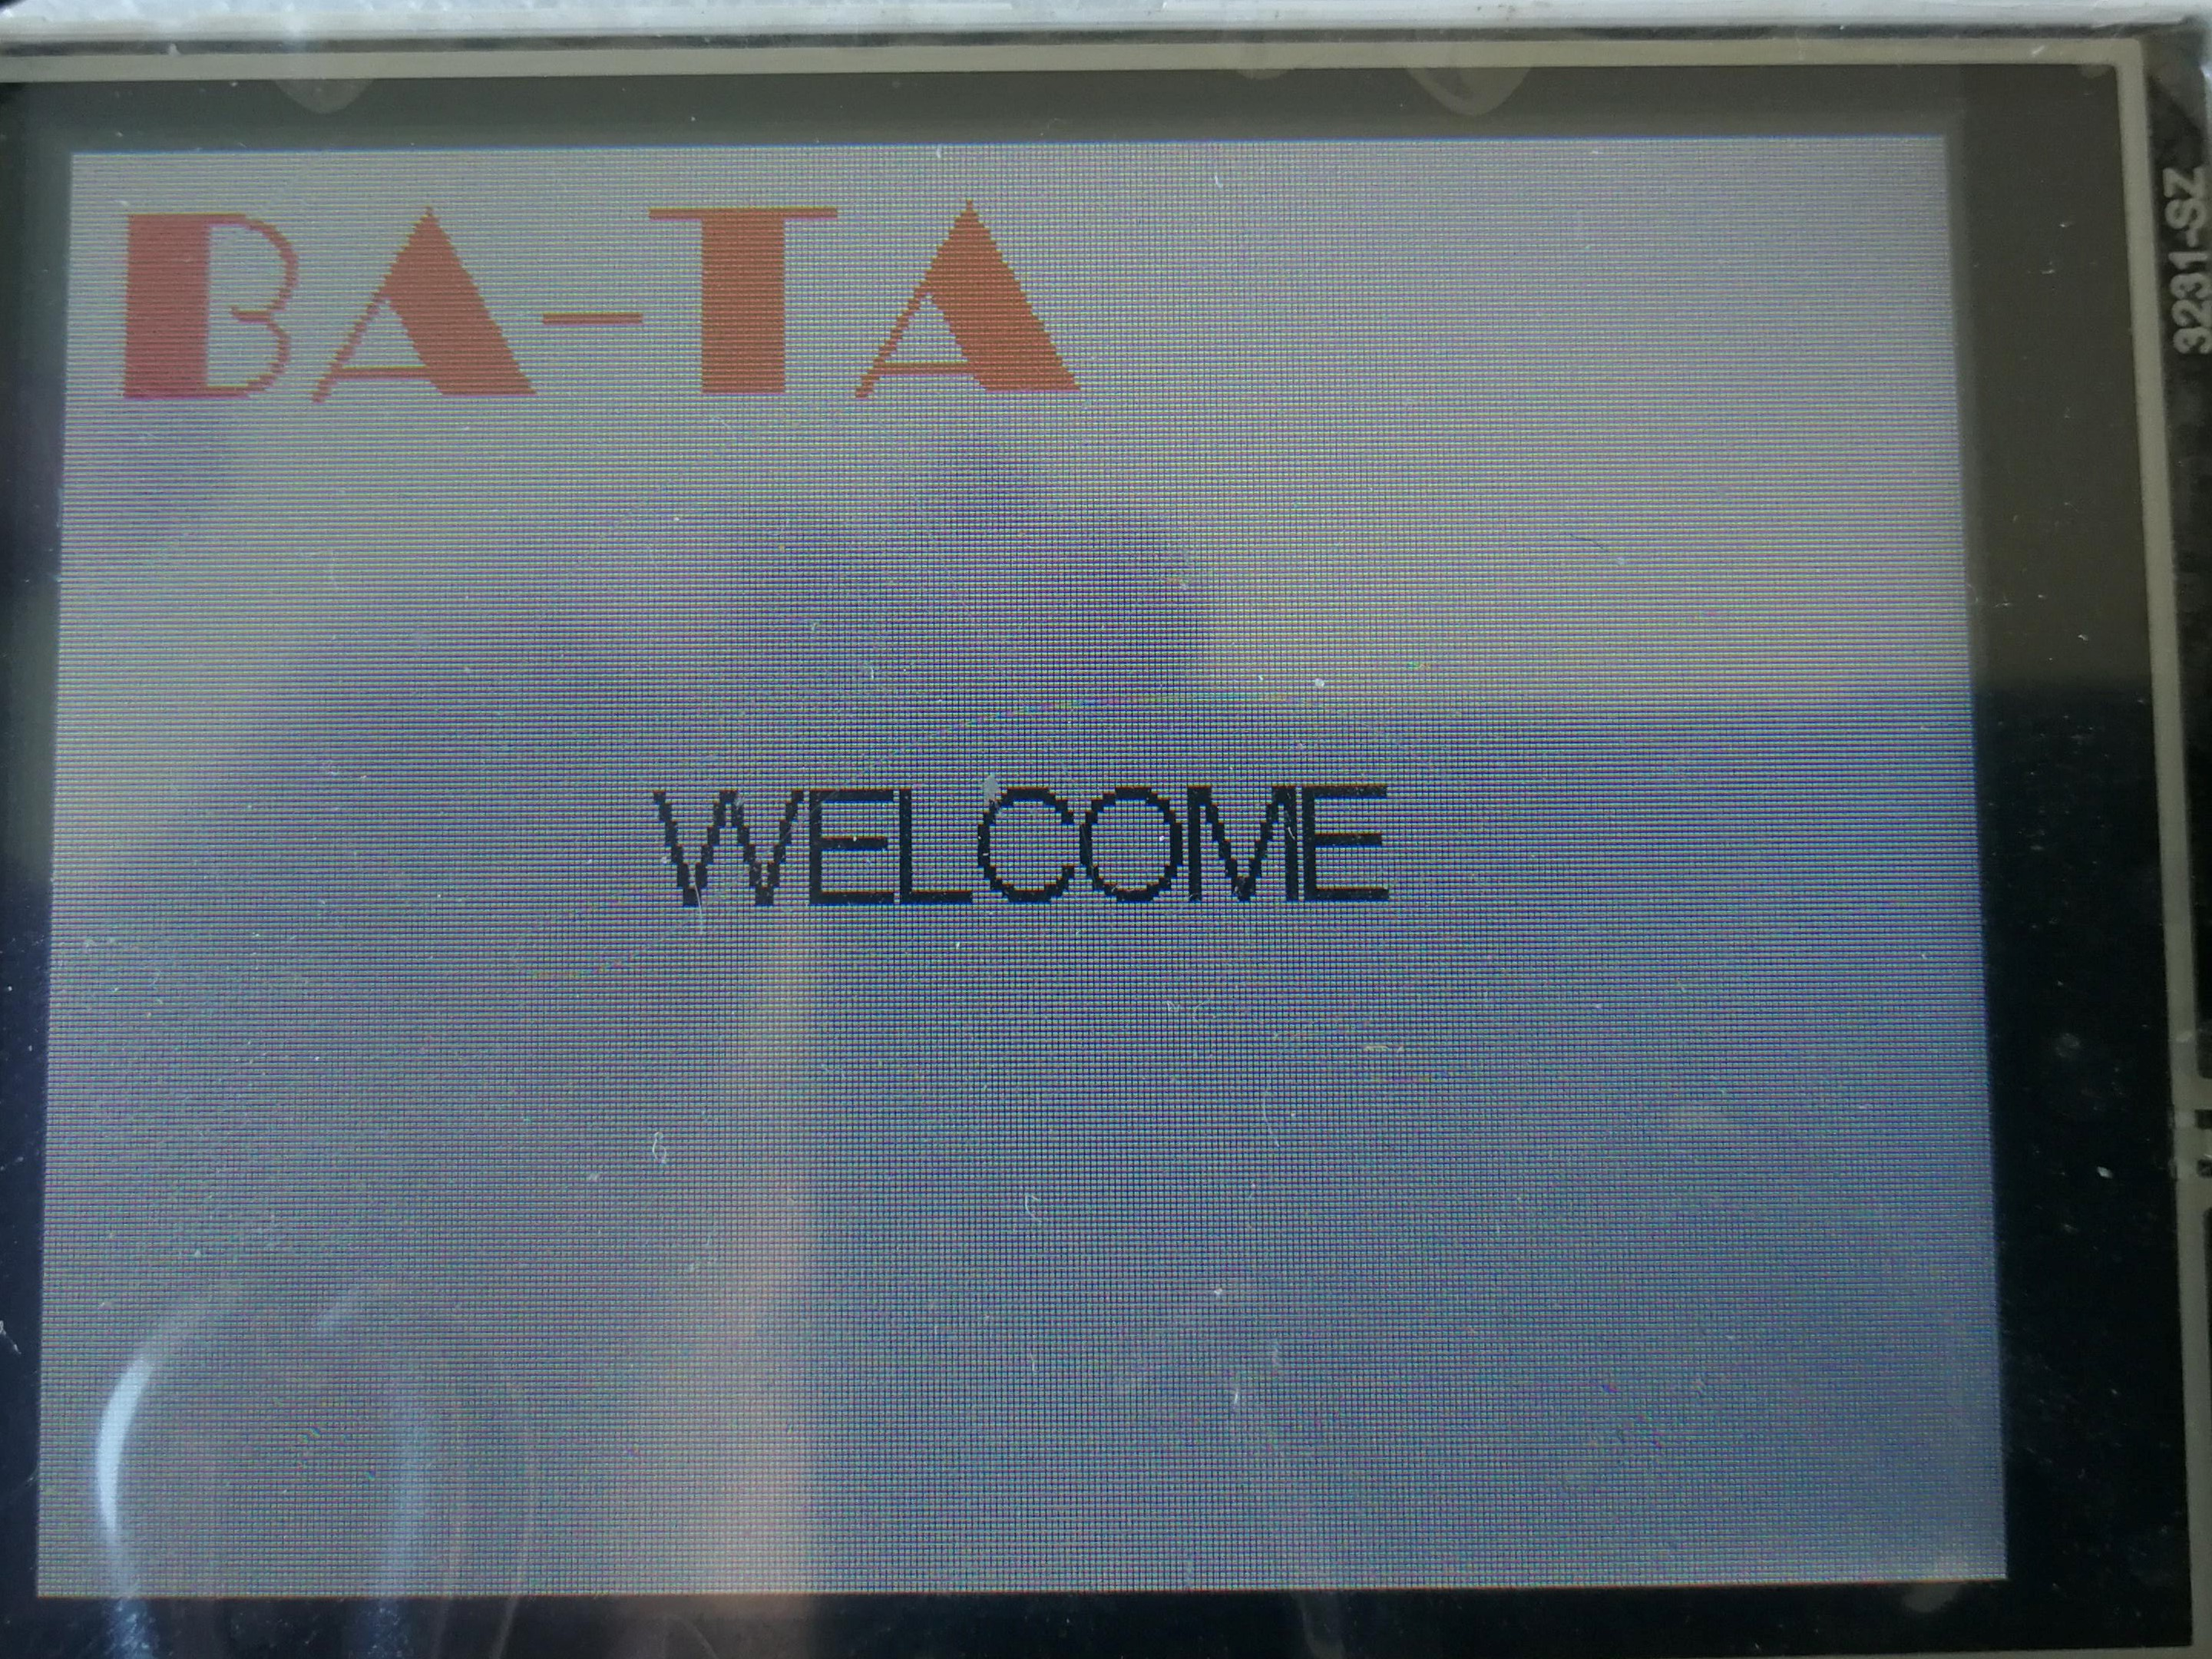
\includegraphics[width = 300 pt]{Img/welcome.jpg}
	\caption{welcome}
	\label{fig:welcome}
\end{figure}
Næste display er en hovedmunu, hvor der er tre forskellige muligheder, som ses på \\figur     \ref{fig:start}. Hertil tilføjes 4 trykknapper, hvor brugeren kan integere med systemet. Med "Enter" vælger brugeren en funktion. "Back" gør brugeren i stand til at gå tilbage til hovedmenuen, hvis man åbner en af de kommene states. "Up" og "Down" flytter pointeren hhv. op og ned. Herudover laves en lås øverst i højre hjørne. Denne lås viser grøn ved låst op og rød ved låst. Øverst til venstre på skærmen vises projektets logo.    
\begin{figure}[H]
	\centering
	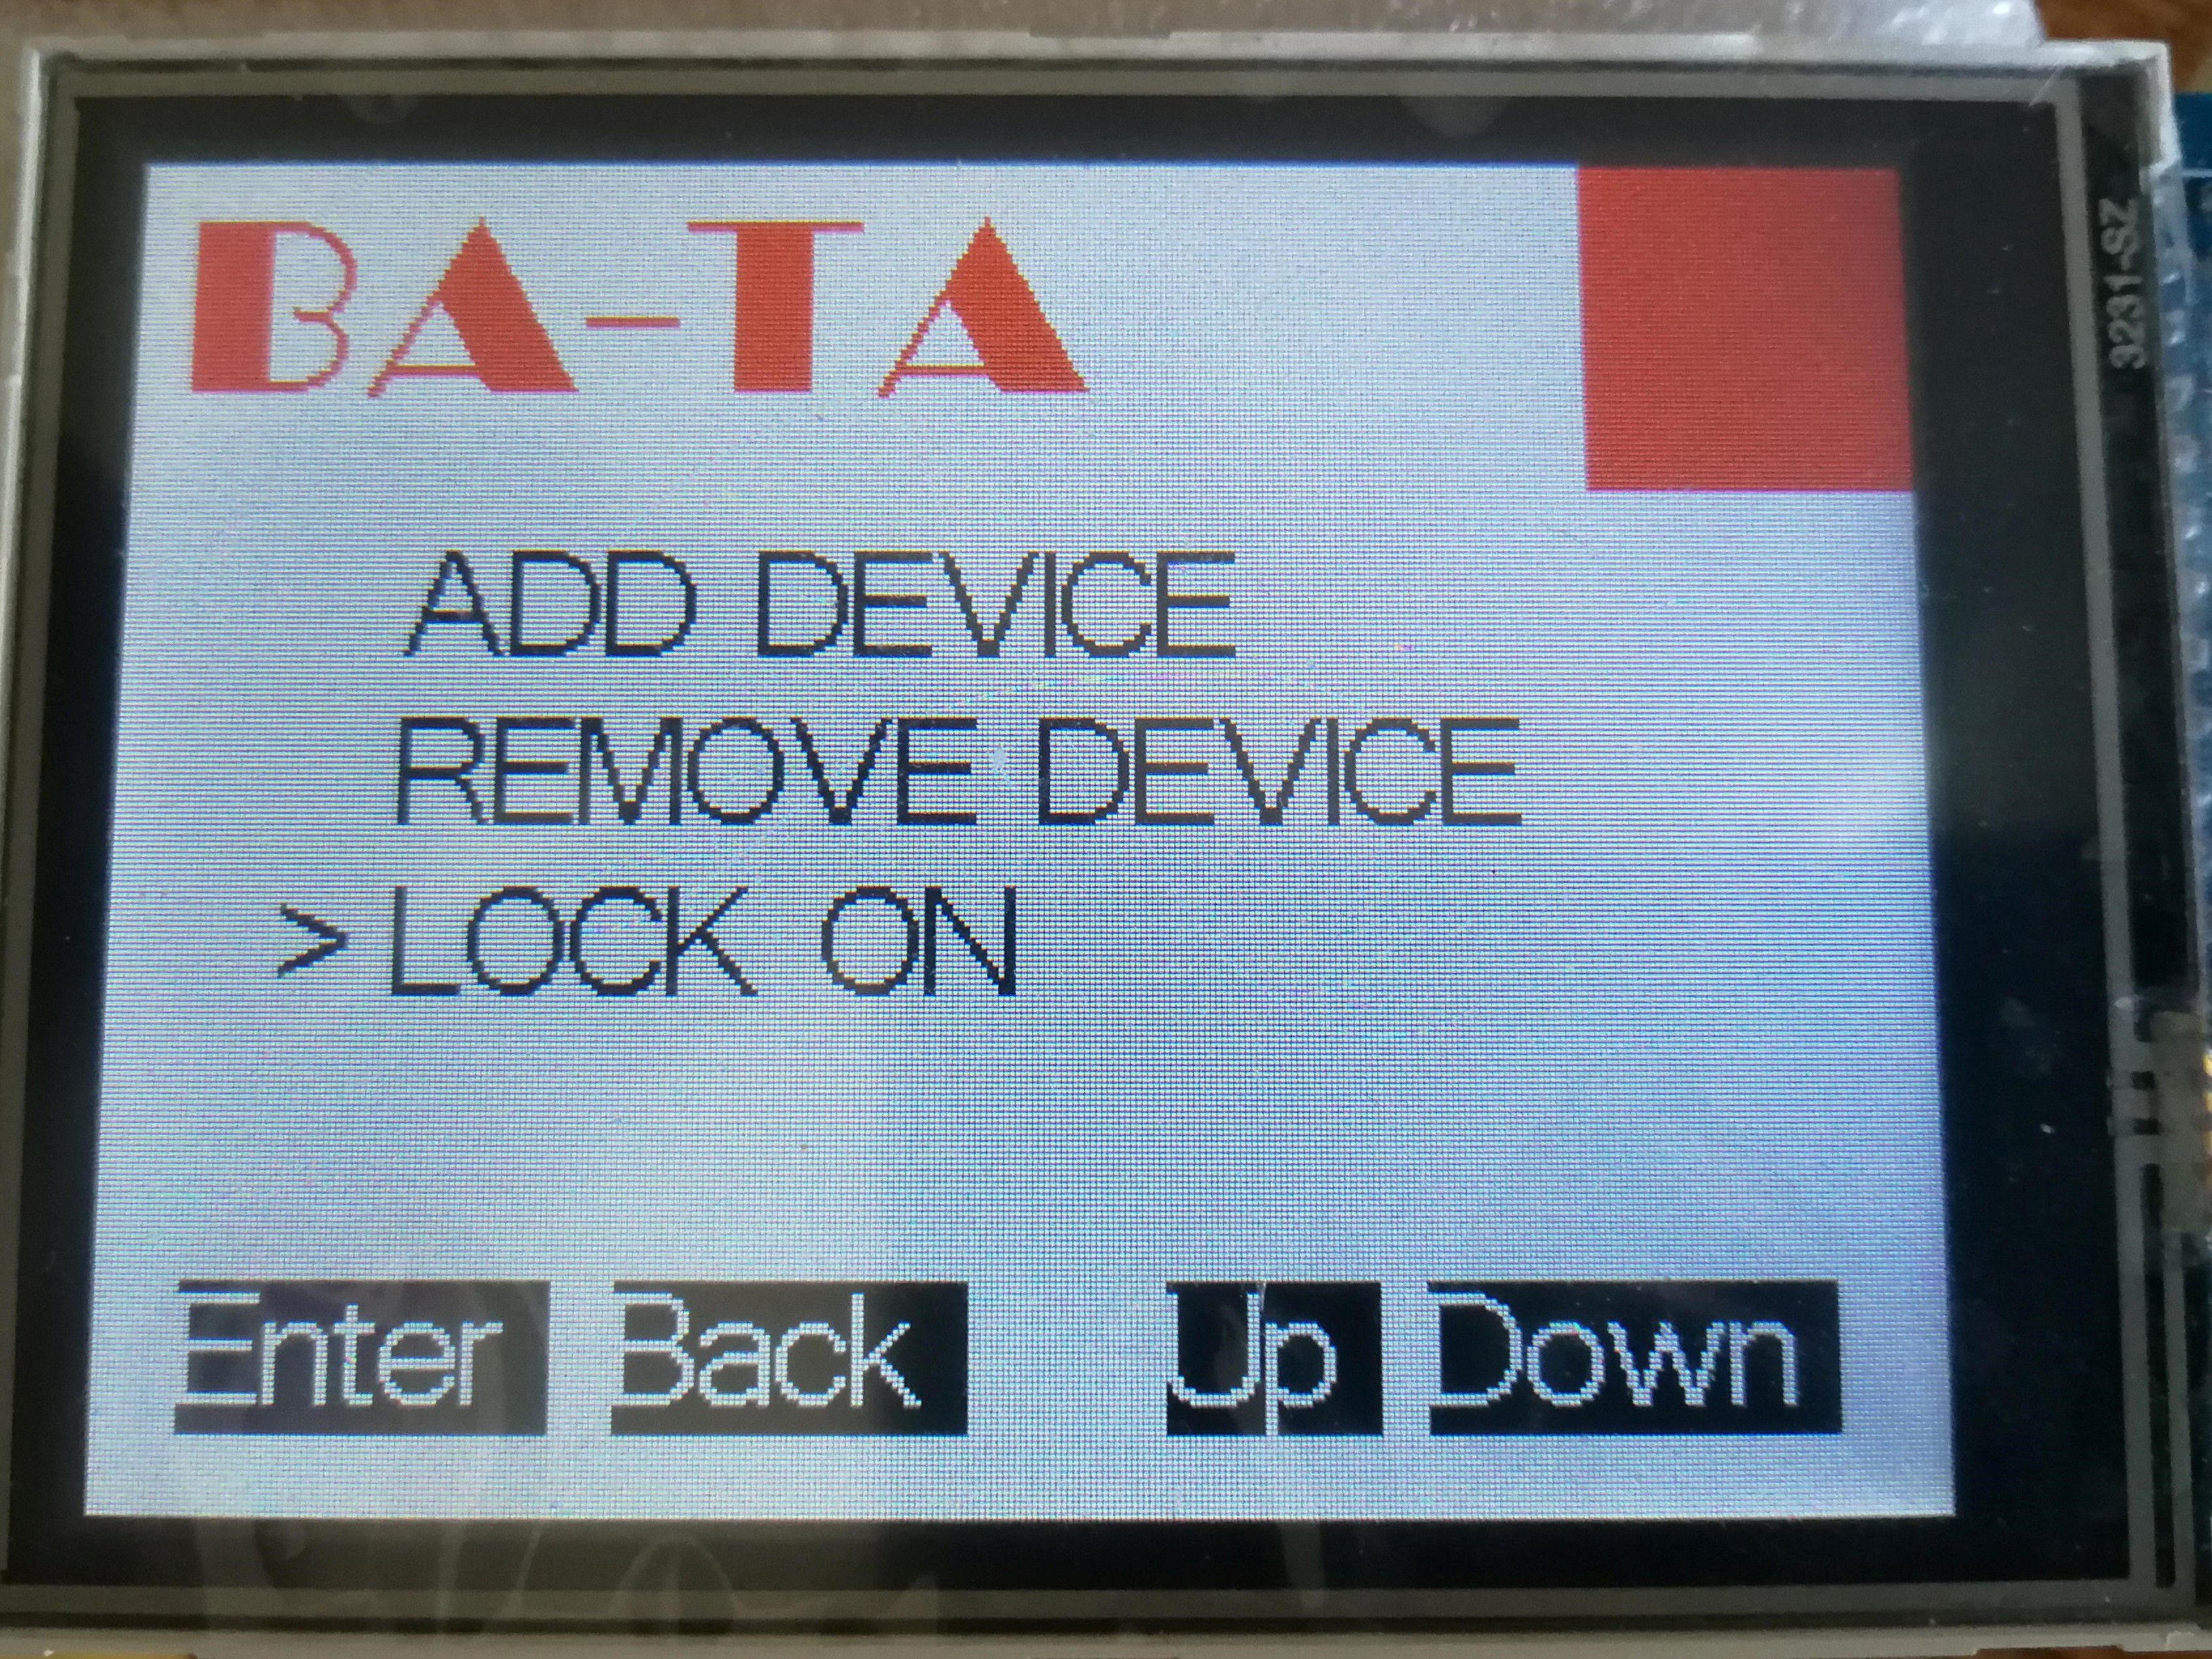
\includegraphics[width = 300 pt]{Img/start.jpg}
	\caption{Hoved Menu}
	\label{fig:start}
\end{figure}

Hvis brugeren trykker på "ADD DEVICE" søger BA-TA efter de 4 stærkeste Bluetooth signaler i nærheden. 
\begin{figure}[H]
	\centering
	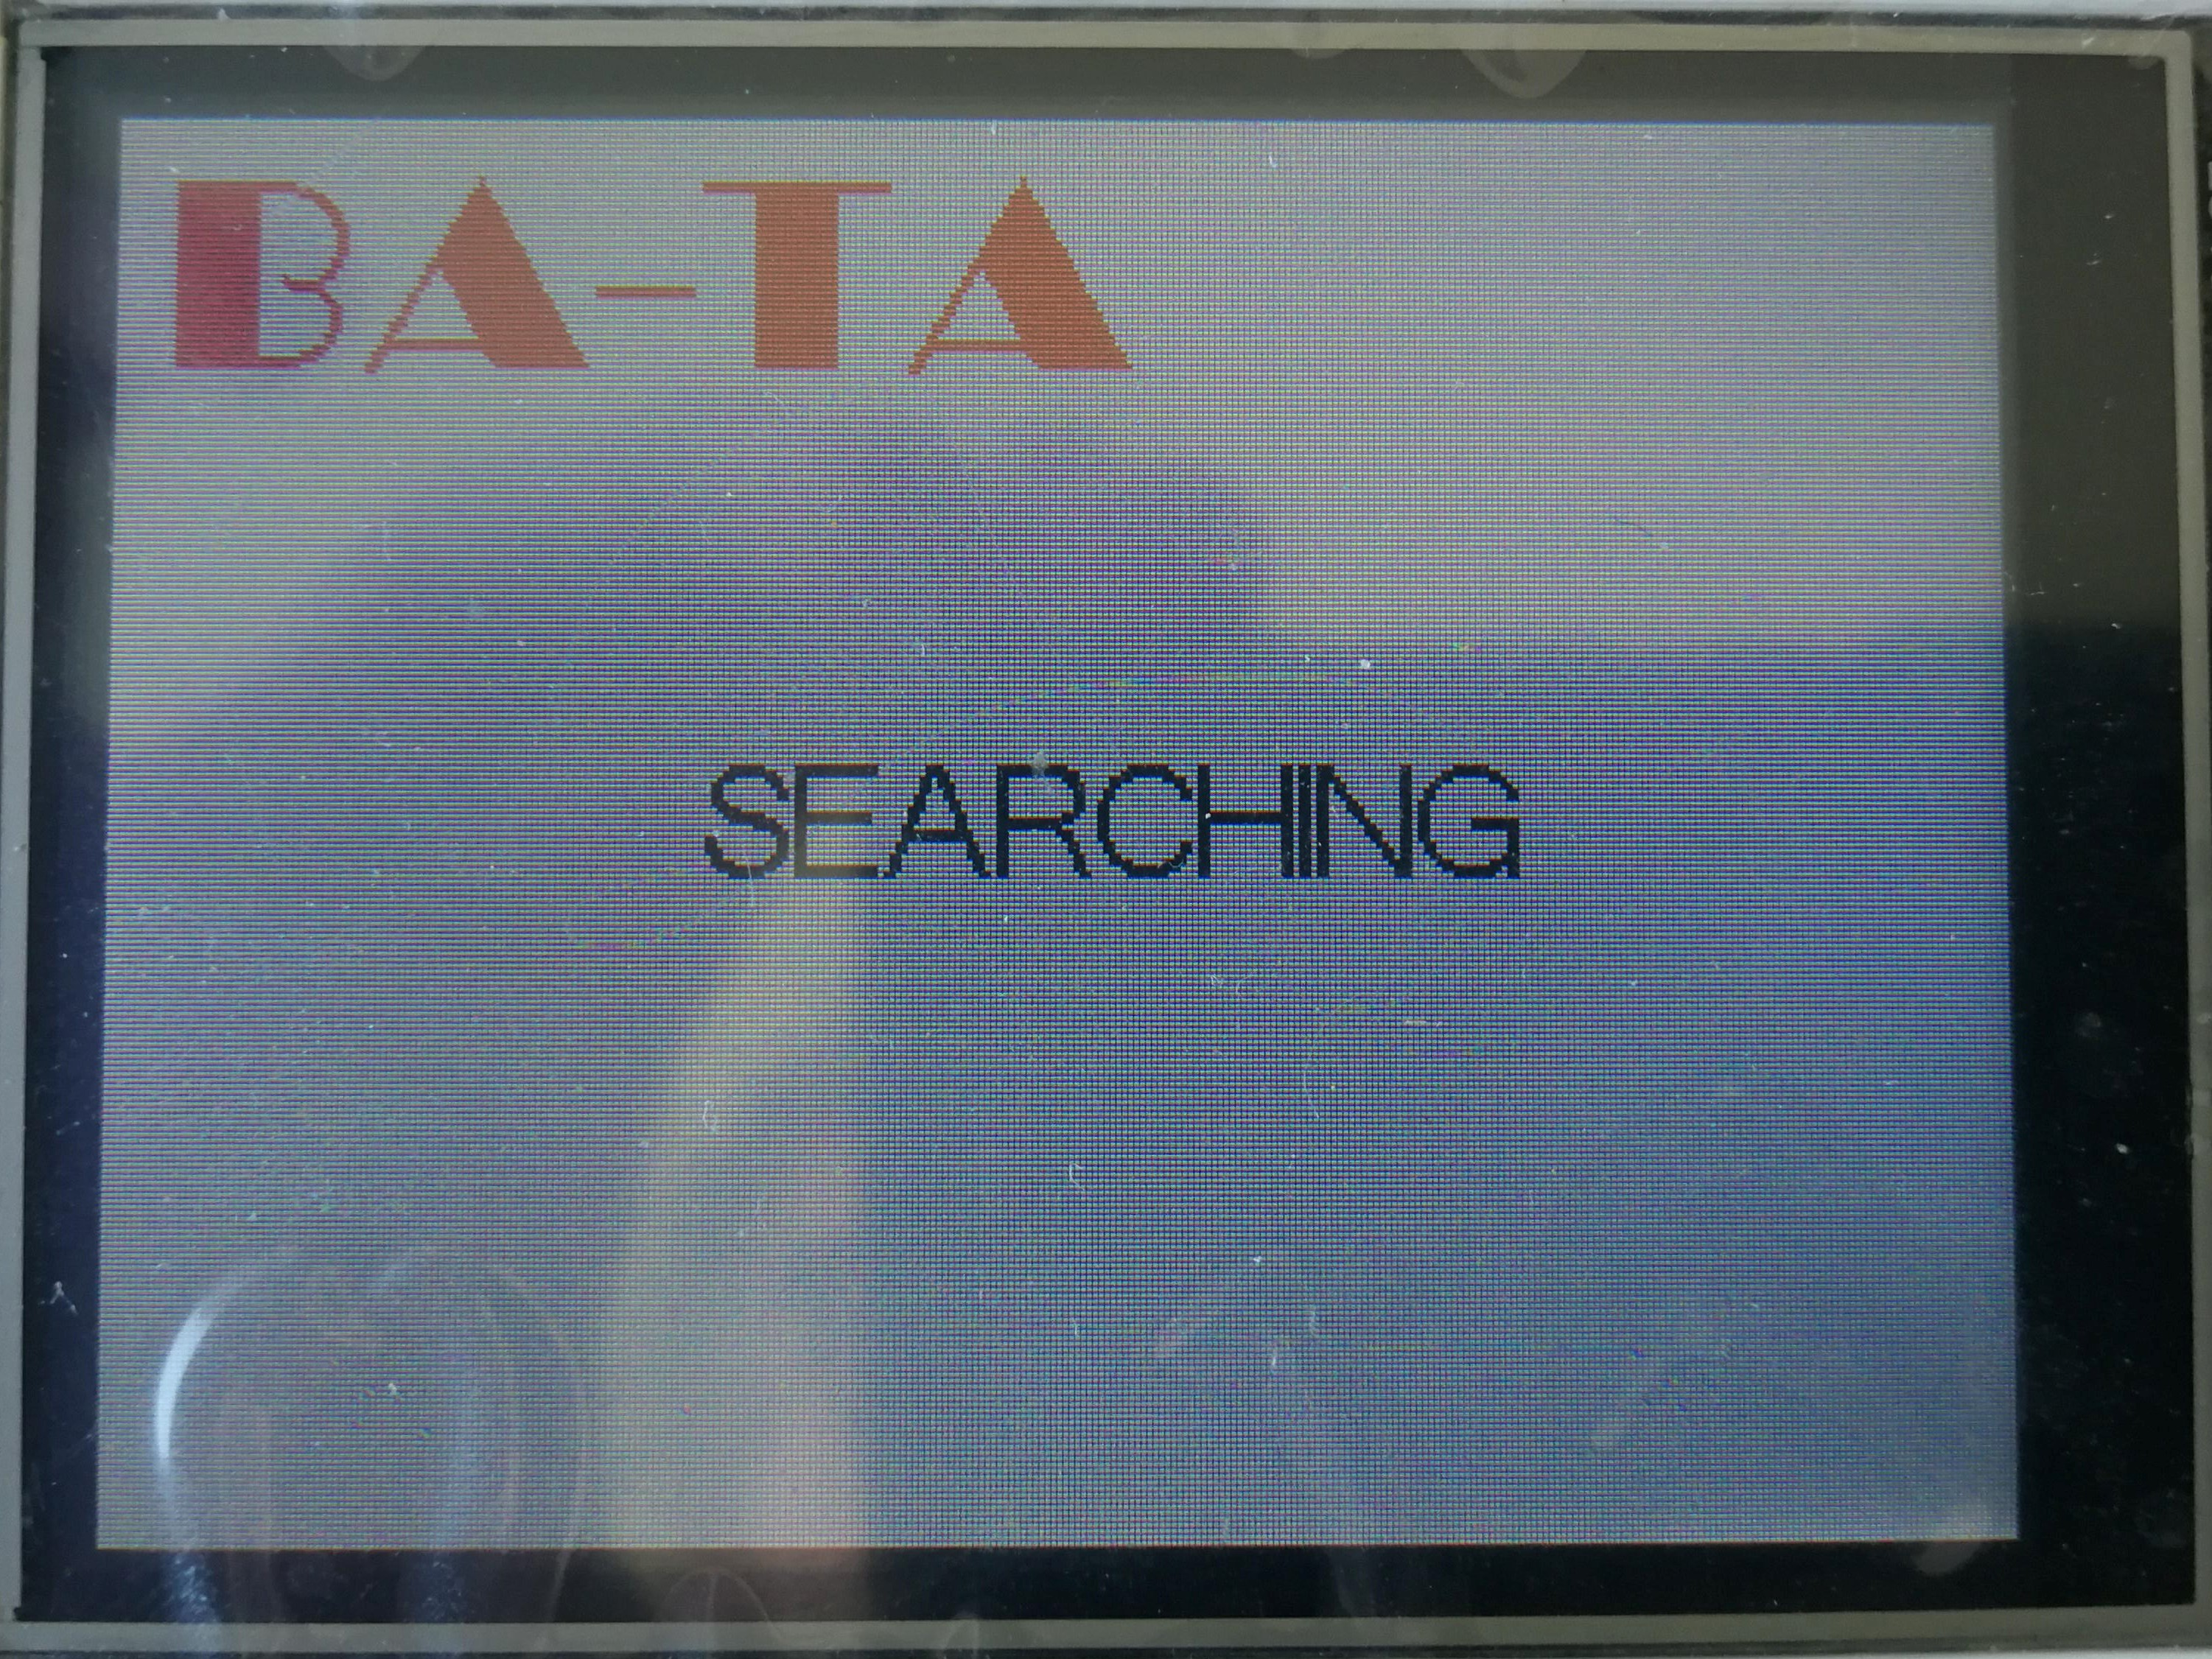
\includegraphics[width = 300 pt]{Img/Searching.jpg}
	\caption{Searching}
	\label{fig:Searching}
\end{figure}
Herefter vises de enheder som kan vælges til systemet. Dette ses på figur \ref{fig:devices}.
\begin{figure}[H]
	\centering
	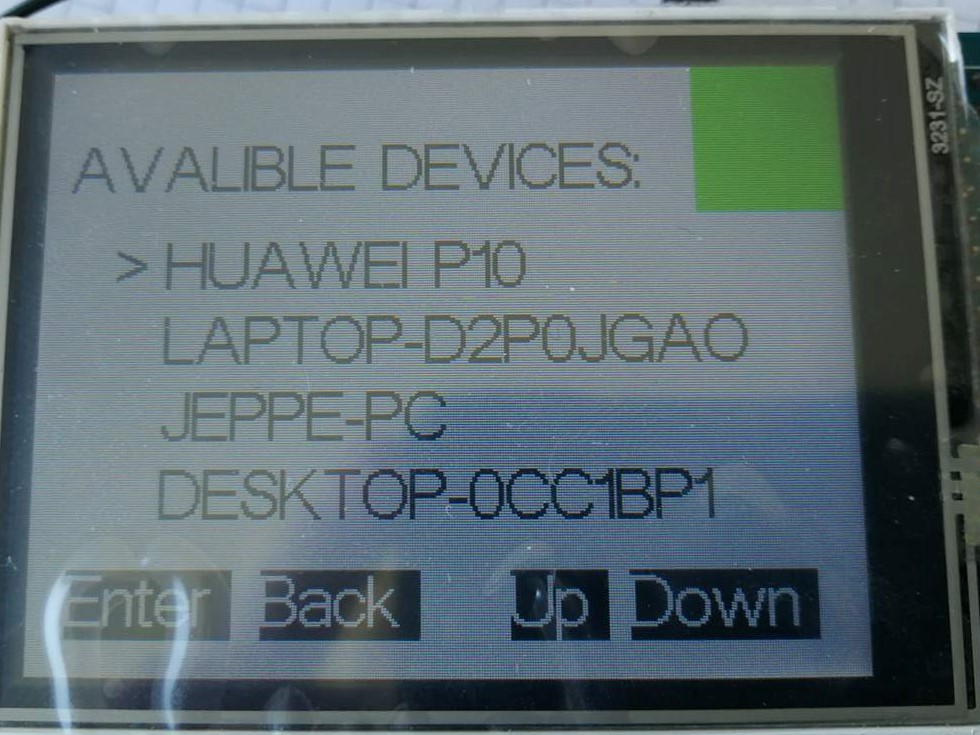
\includegraphics[width = 300 pt]{Img/devices.jpg}
	\caption{Tilgængelige enheder}
	\label{fig:devices}
\end{figure}
Hvis der vælges en enhed, viser displayet hvilken enhed der er valgt. 
\begin{figure}[H]
	\centering
	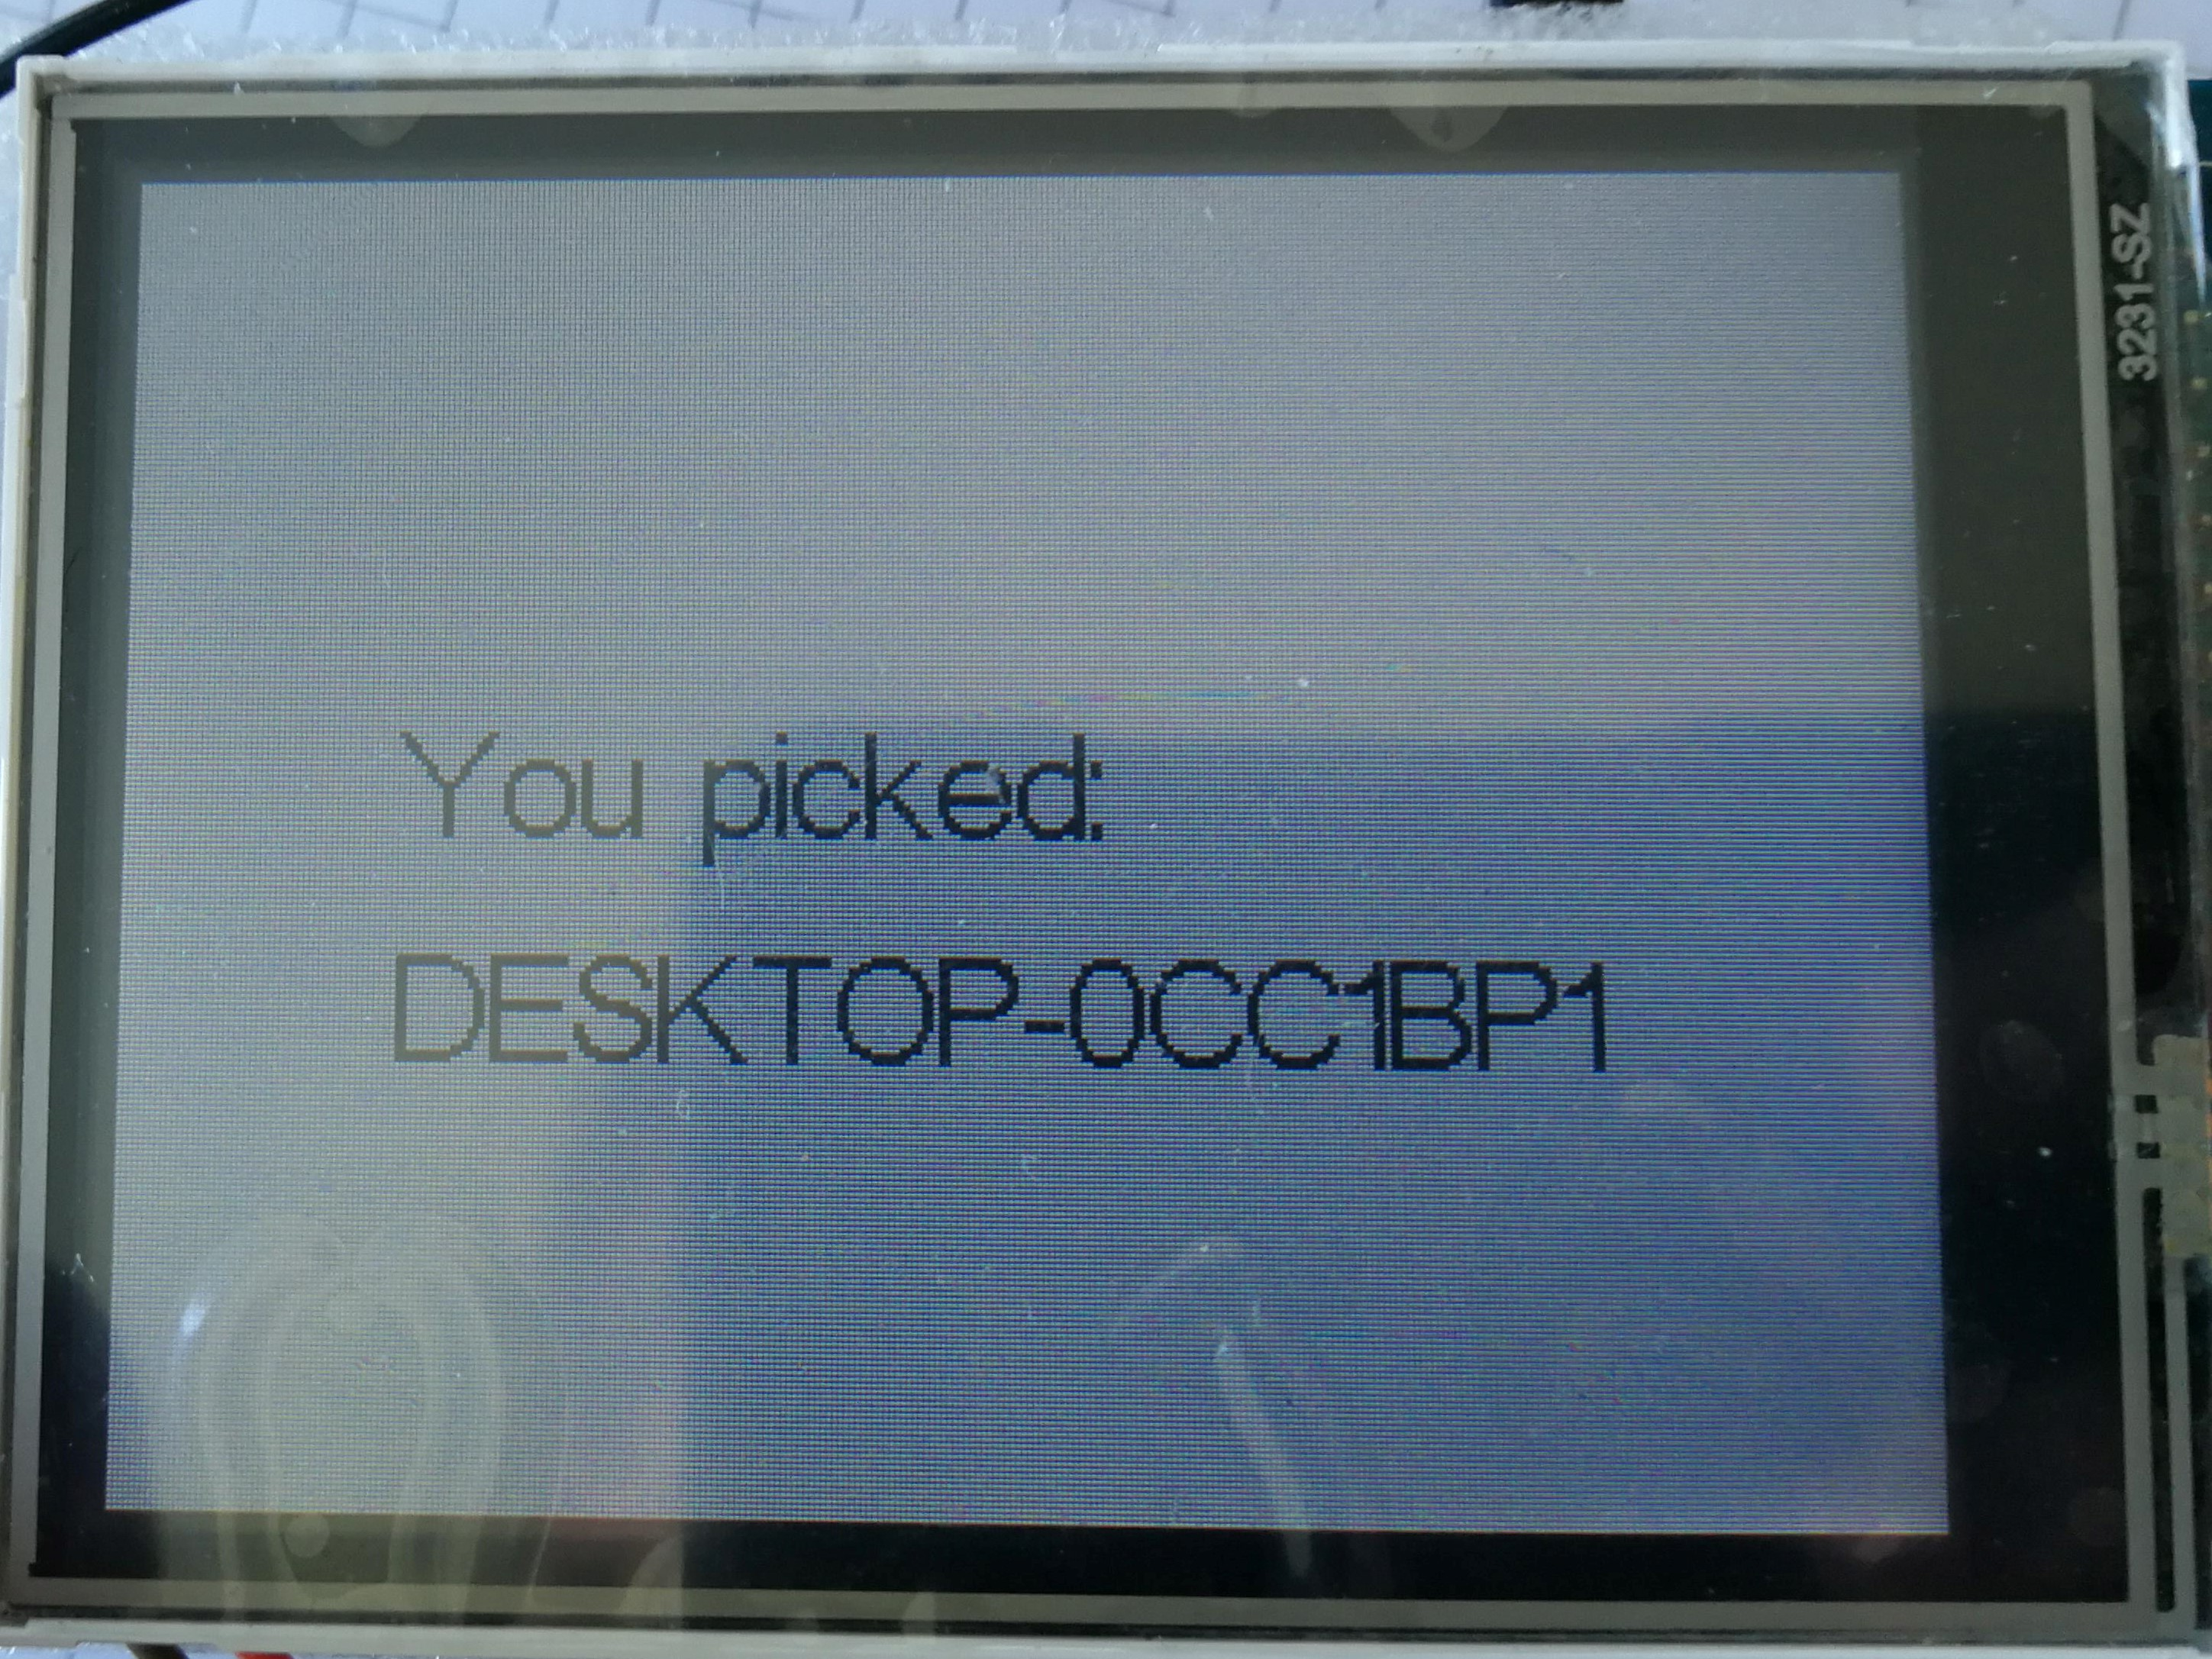
\includegraphics[width = 300 pt]{Img/pick.jpg}
	\caption{Valg af enhed}
	\label{fig:pick}
\end{figure}
Hvis brugeren herefter vælger funktionen "REMOVE DEVICE" fra figur \ref{fig:start}, åbnes hvilke enheder der er gemt Dette ses på \ref{fig:remove}.. Hvis der ikke er gemt nogen device, er displayet tomt, som vises på figur \ref{fig:noDevices}. 
\begin{figure}[H]
	\centering
	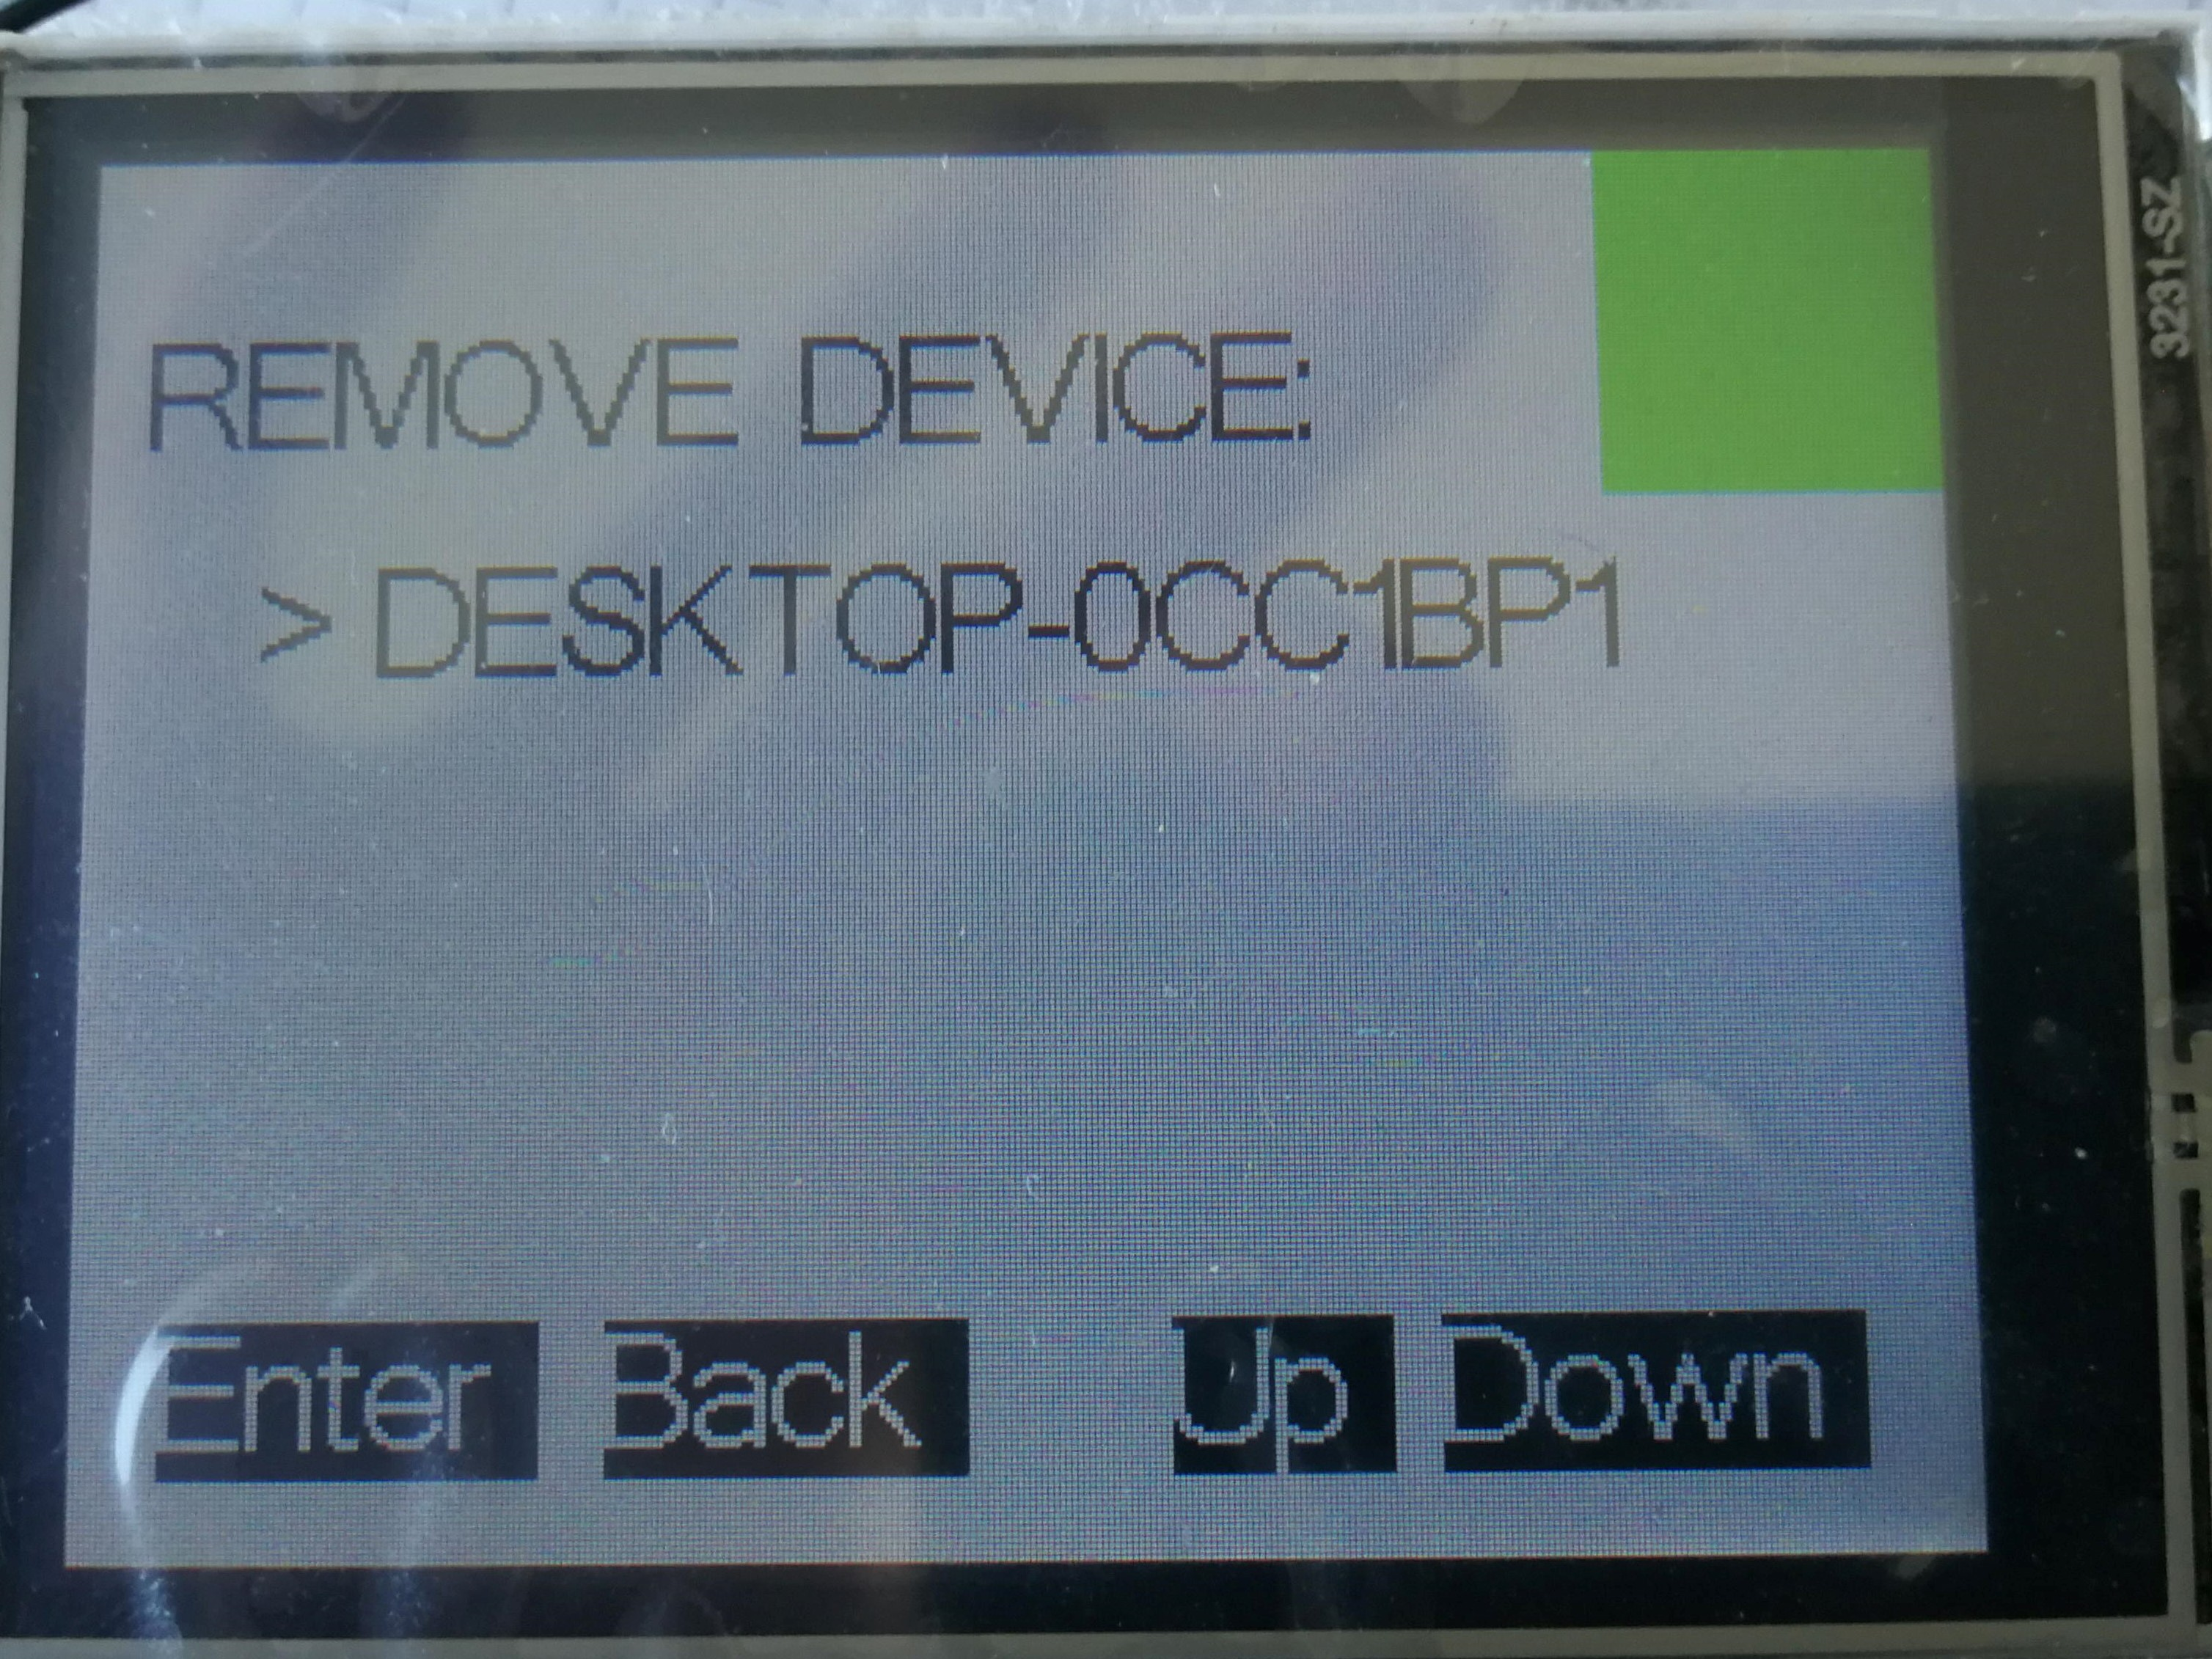
\includegraphics[width = 300 pt]{Img/remove.jpg}
	\caption{Fjern en enhed}
	\label{fig:remove}
\end{figure}
\begin{figure}[H]
	\centering
	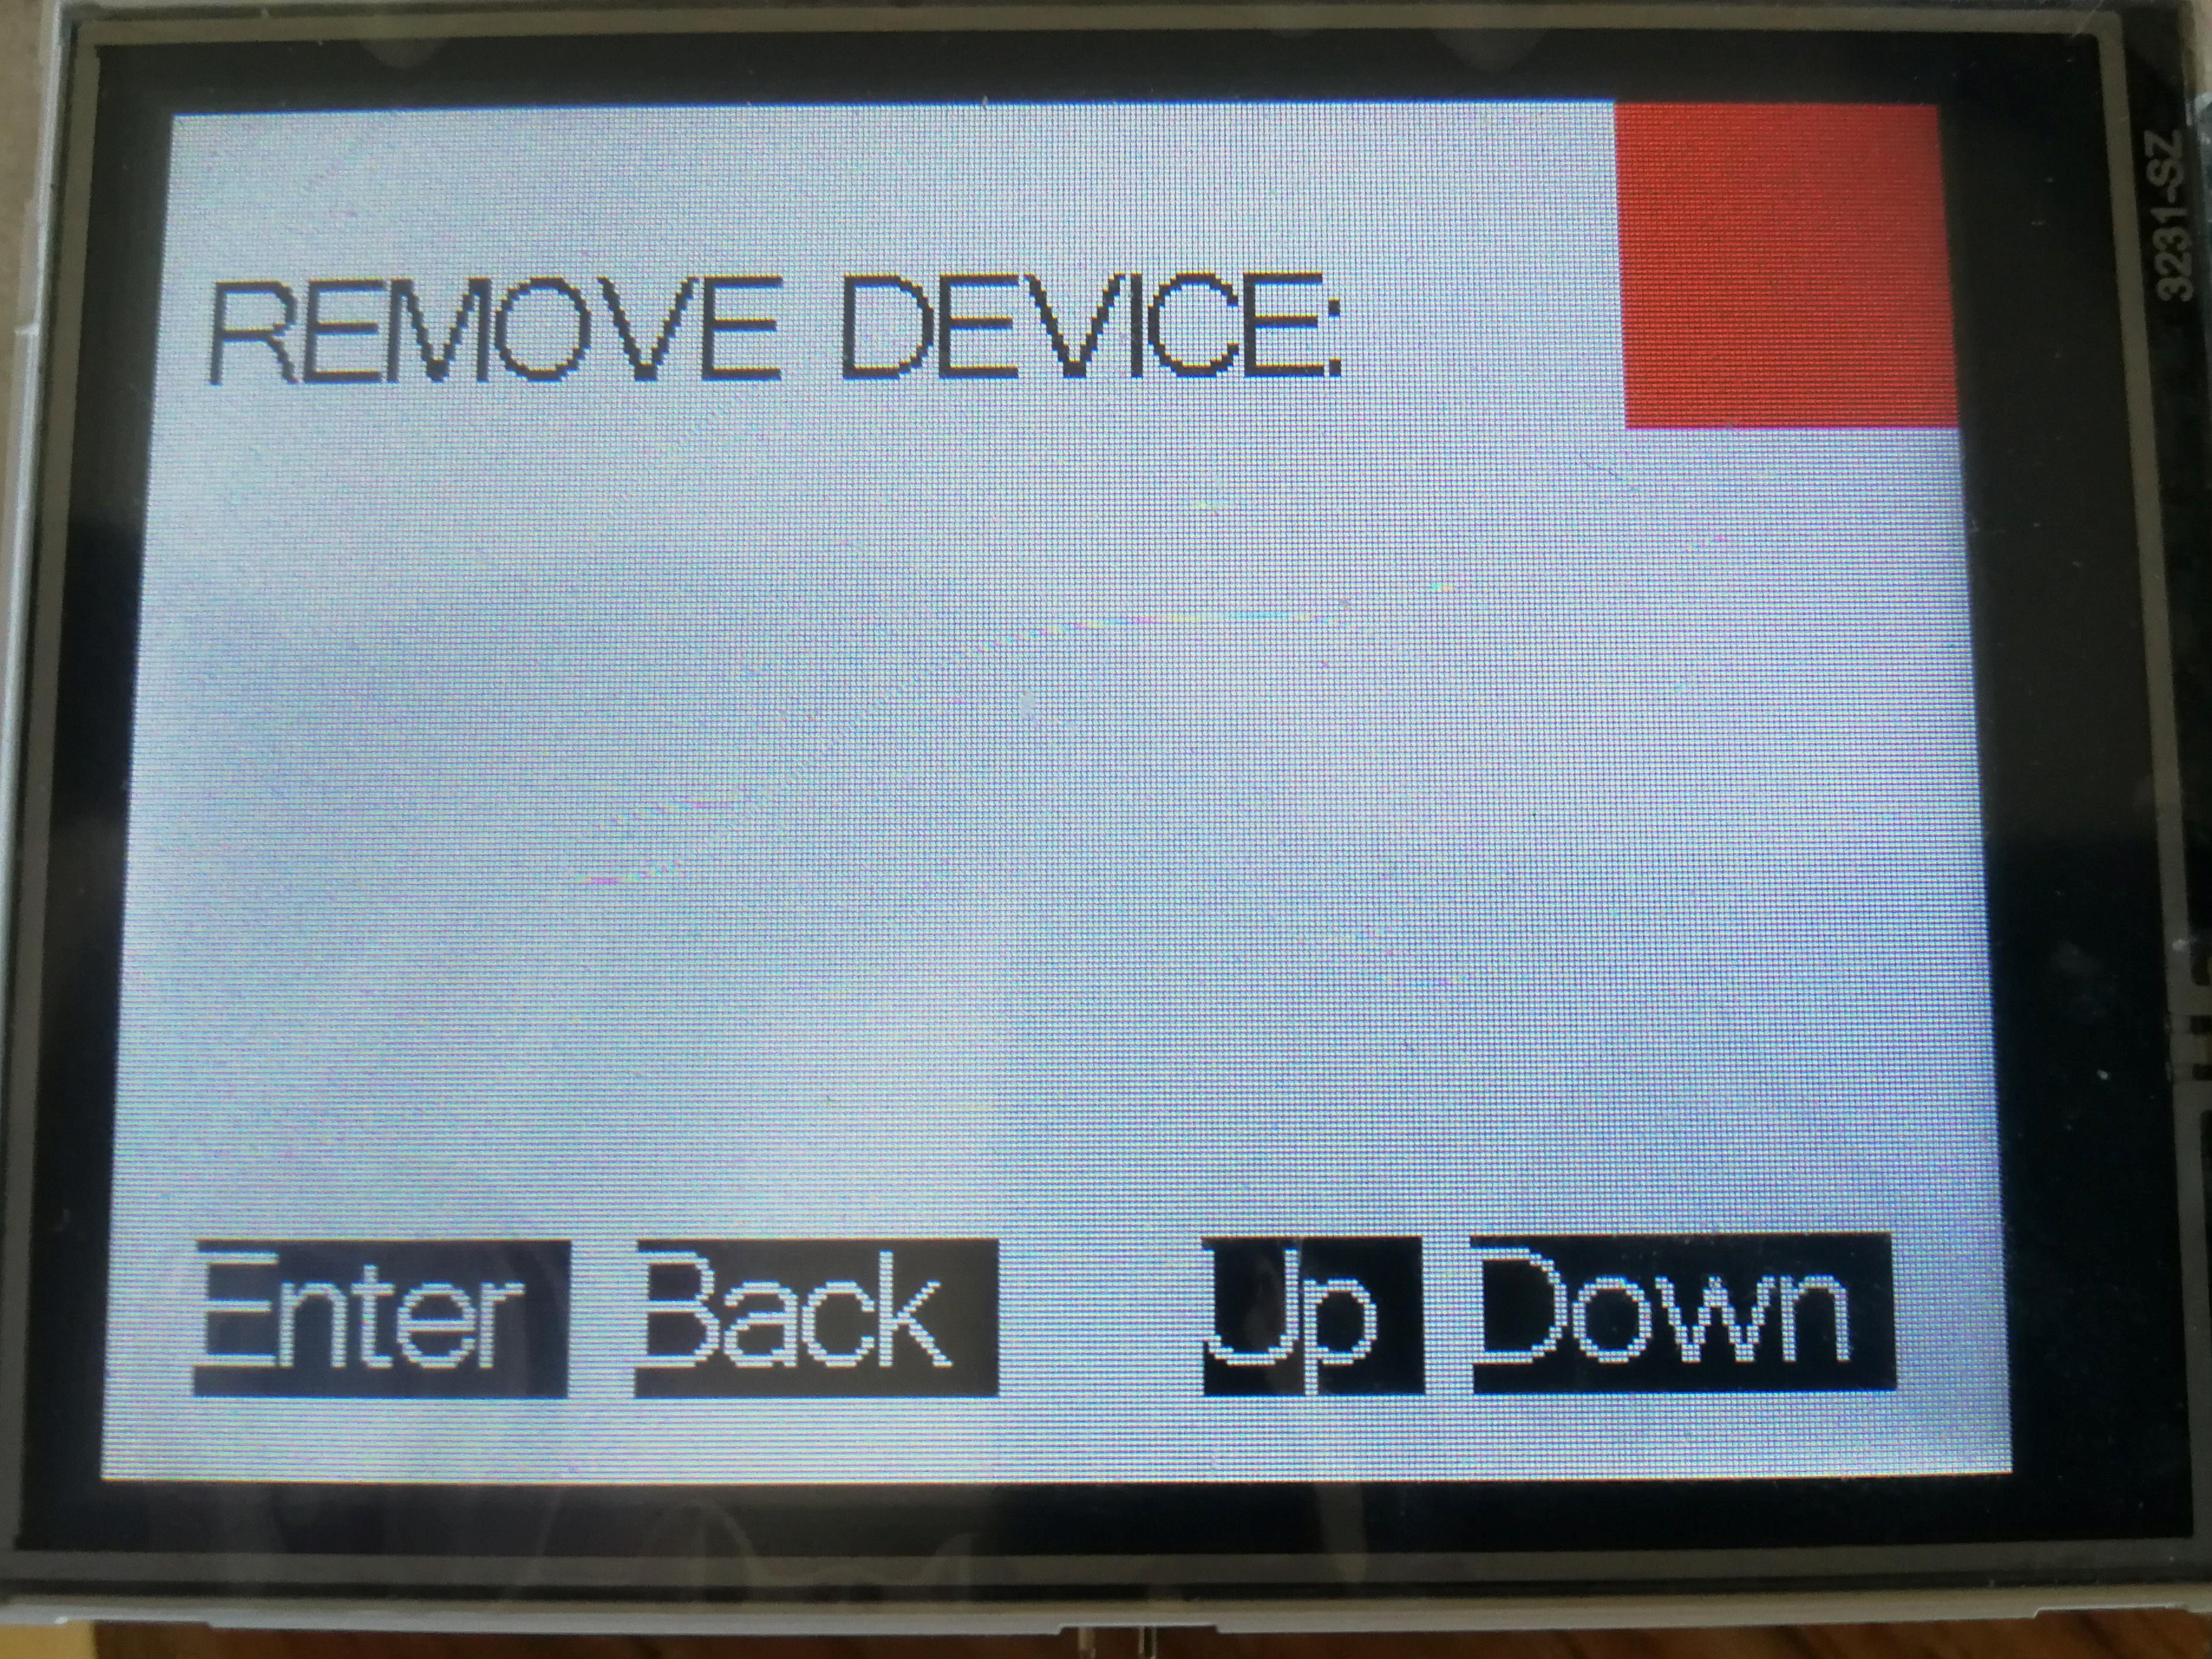
\includegraphics[width = 300 pt]{Img/noDevice.jpg}
	\caption{Ingen enehder}
	\label{fig:noDevices}
\end{figure}
Herefter kan brugeren vælge at slette en bestemt enhed. Dette sker ved at trykke "Enter" ved den rette enhed. Displayet viser på figur \ref{fig:delete} en besked om hvilken enhed der er slettet. 
\begin{figure}[H]
	\centering
	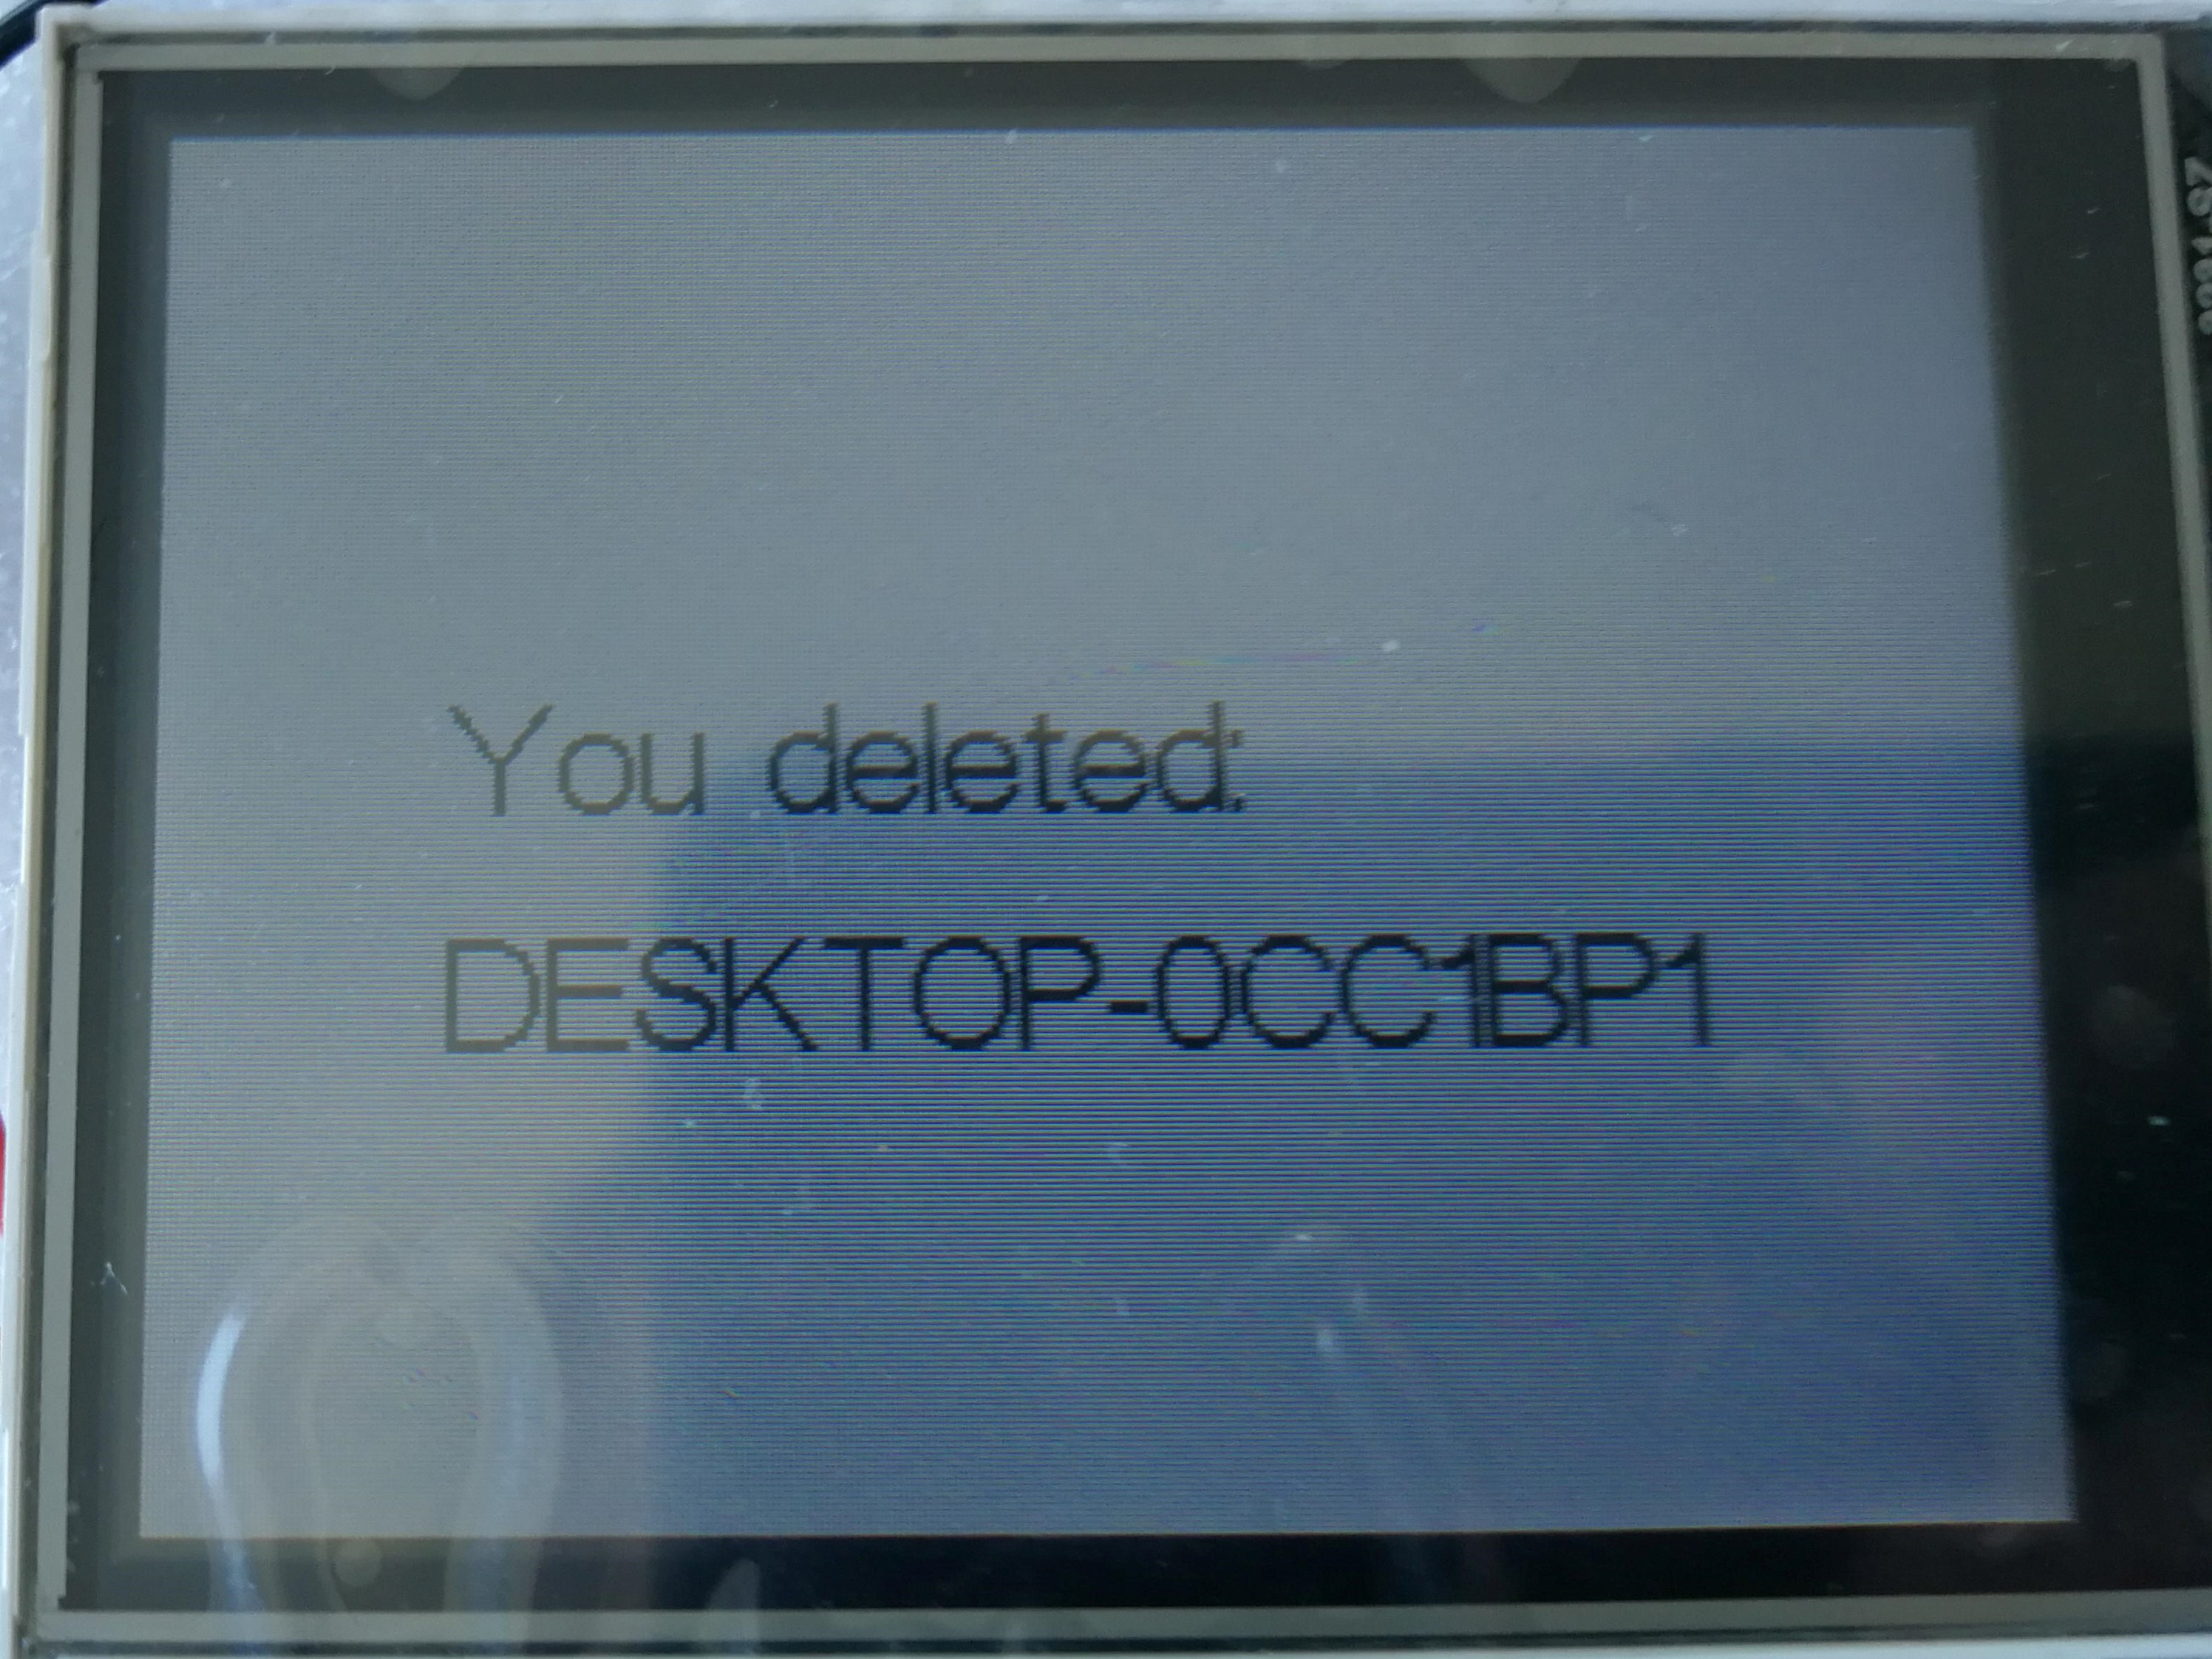
\includegraphics[width = 300 pt]{Img/delete.jpg}
	\caption{Valgt fjernet en enhed}
	\label{fig:delete}
\end{figure}
Hvis brugeren trykker på den sidste state i Hoved Menuen, låses systemet op, teksten skifter og låsen skifter farve. Dette ses på \ref{fig:lockOff}.
\begin{figure}[H]
	\centering
	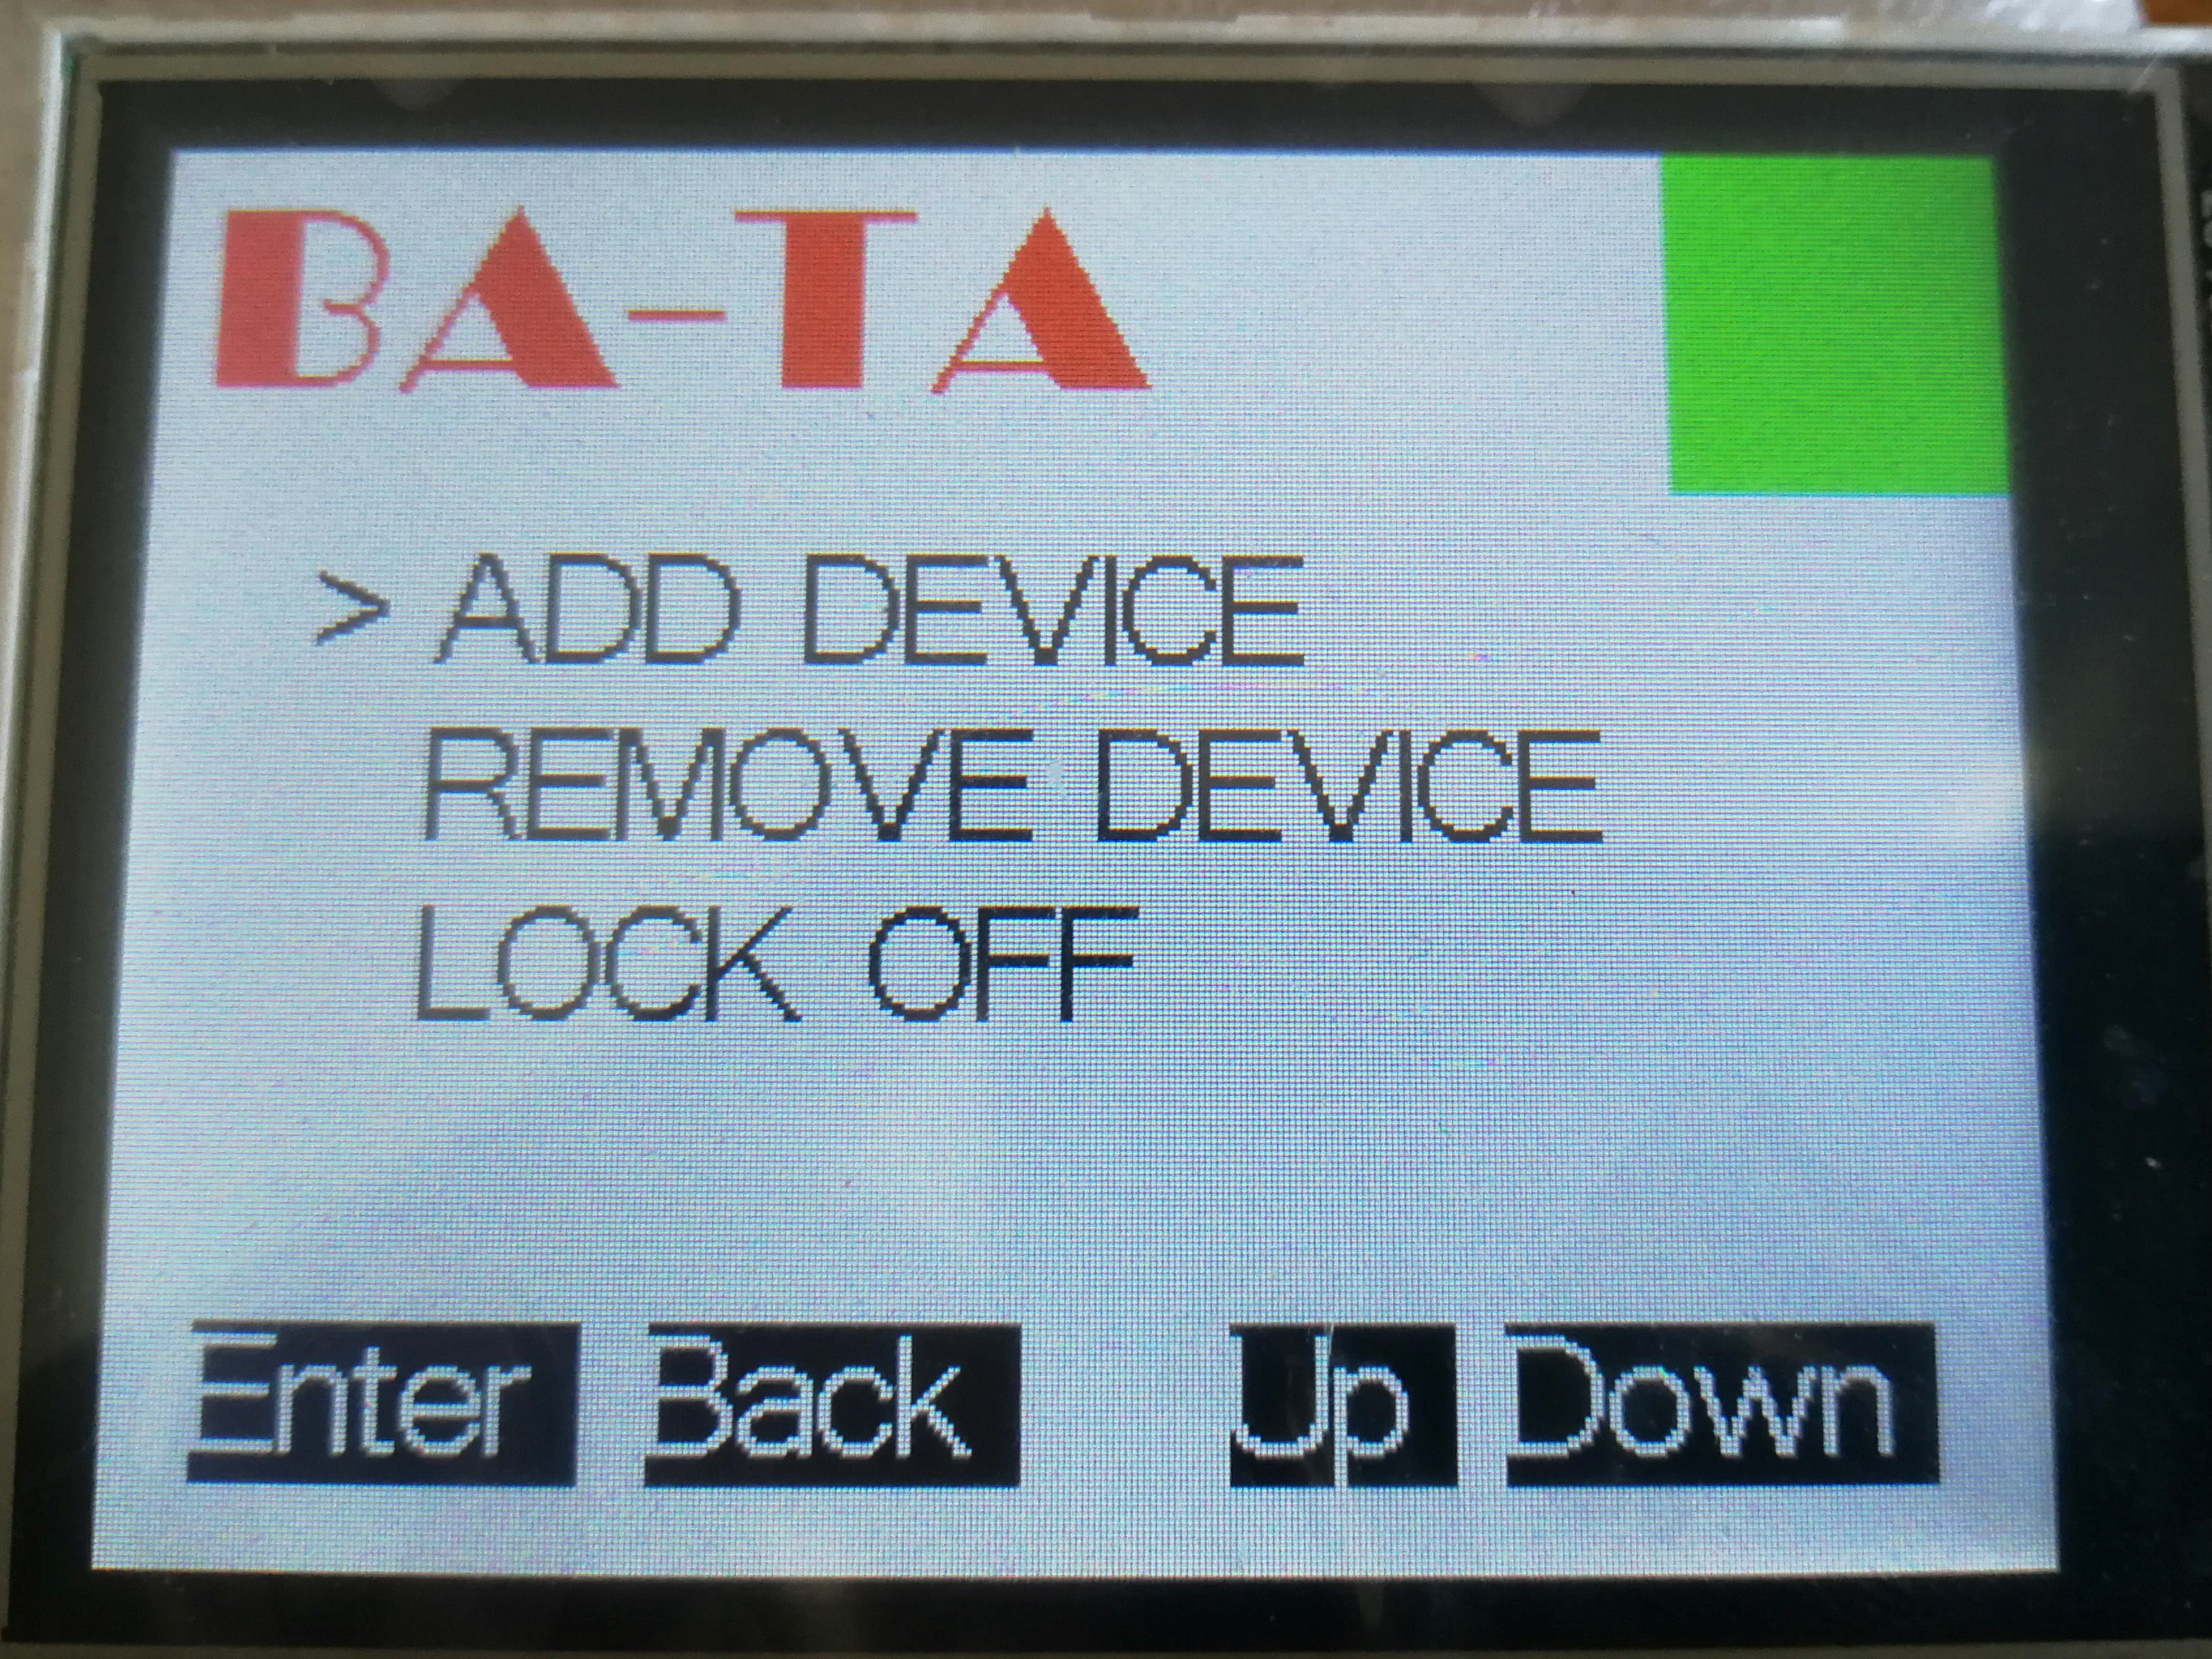
\includegraphics[width = 300 pt]{Img/lockOff.jpg}
	\caption{Låst op}
	\label{fig:lockOff}
\end{figure}
Hvis der endnu engang trykkes på den sidste state i Hoved Menuen, ændres teksten, og låsen skifter, alt efter BA-TA's funktionalitet. Hvis der trykkes endnu engang på sidste state, ændres låsen til default, som er låst. 
\begin{figure}[H]
	\centering
	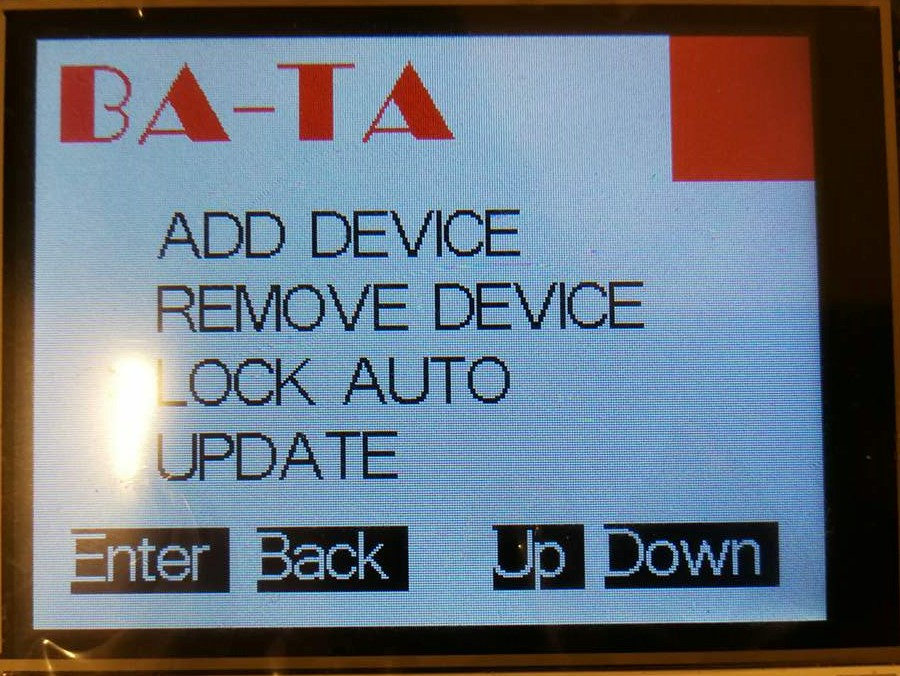
\includegraphics[width = 300 pt]{Img/auto.jpg}
	\caption{Lås Automatisk}
	\label{fig:auto}
\end{figure}

